\documentclass[10pt]{exam}
\usepackage[hon]{template-for-exam}
\usepackage{tikz}

\title{Vector Addition (Consolidation)}
\author{Rohrbach}
\date{\today}

\begin{document}
\maketitle

\noindent
Vectors $\vec{A}$ and $\vec{B}$ are shown below.

\vspace{2em}

  \begin{parts}
    \part 
      Find the components of $\vec{A}$ and $\vec{B}$.
    \part
      Sketch out what $\vec{R}=\vec{A}-2\vec{B}$ would look like. 
    \part
      Calculate the magnitude and direction of $\vec{R}$
  \end{parts}

  \vspace{1em}

  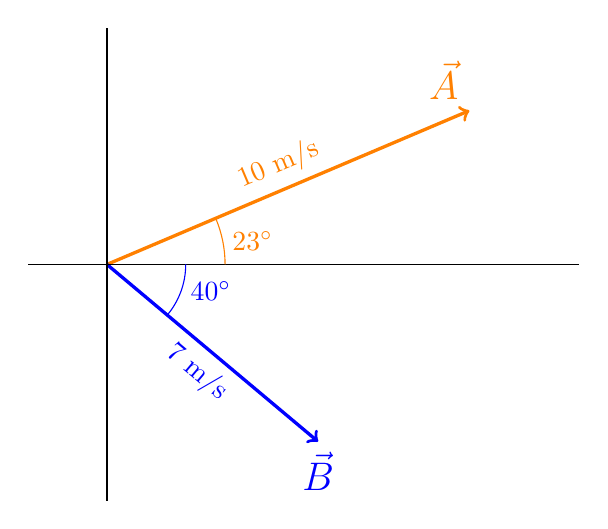
\begin{tikzpicture}[
    vector/.style={
      ->,
      very thick,
    }
  ]
    \def\unit{0.5}
    

    \draw[vector,orange] (0,0) -- (23:10*\unit) 
      node[anchor=south east] {\Large $\vec{A}$} 
      node[midway,above,rotate=23] {10 m/s};
    \draw[vector,blue] (0,0) -- (-40:7*\unit)
      node[anchor=north] {\Large $\vec{B}$}
      node[midway,below,rotate=-40] {7 m/s};
    \draw (0,3) -- (0,-3);
    \draw (-1,0) -- (6,0);

    \draw[orange] (1.5,0) arc (0:23:1.5) 
      node[midway,right] {$23^\circ$};
    \draw[blue] (1,0) arc (0:-40:1) 
      node[midway,right] {$40^\circ$};



  \end{tikzpicture}

\end{document}